\documentclass[conference]{IEEEtran}
\IEEEoverridecommandlockouts
\usepackage{cite}
\usepackage{amsmath,amssymb,amsfonts}
\usepackage{algorithmic}
\usepackage{graphicx}
\usepackage{textcomp}
\usepackage{xcolor}
\usepackage{hyperref}
\usepackage{float}

\graphicspath{ {diagrams/} }

\def\BibTeX{{\rm B\kern-.05em{\sc i\kern-.025em b}\kern-.08em
    T\kern-.1667em\lower.7ex\hbox{E}\kern-.125emX}}
\begin{document}

\title{Implementácia disassebleru pre architektúru OpenRISC 1000}

\author{\IEEEauthorblockN{Jakub Dubec}
\IEEEauthorblockA{\textit{Ústav počítačového inžinierstva a aplikovanej informatiky} \\
\textit{Fakulta informatiky a informačných technológií STU v Bratislave}\\
Bratislava, Slovakia \\
jakub.dubec@gmail.com}
}

\maketitle

\begin{abstract}
Tento dokument opisuje návrh a implementáciu spätného prekladača, ktorého vstup sú ELF komplikované pre architektúru OpenRISC 1000. Analyzuje základne opisuje črty spomínanej architektúry a kategorizuje jej inštrukčnú sadu. Budeme sa venovať aj stručnej charakteristike ELF súborov, využívaných na UNIX kompatibilných platformách. Technická realizácia je postavená na aplikačnom rámci Xamarin.macOS a Cocoa (cieľom bolo vytvorenie natívnej stolovej aplikácie).
\end{abstract}

\begin{IEEEkeywords}
openrisc, elf, disassembler, inštrukčné sady, macos, počítačévé architektúry
\end{IEEEkeywords}

\section{Úvod}
Pod pojmom spätný preklad chápeme proces transformácie spustiteľného binárneho súboru do jazyka symbolických inštrukcií. Inštrukčná sada (množina všetkých inštrukcií) je definovaná  počítačovou architektúrou, ktorá opisuje abstraktnú internú organizáciu počítača spolu s opisom jej výpočtových schopností \cite{clements2006principles}. Výrobcovia hardvéru štandardne špecifikujú, ktorú architektúru implementujú pre daný produkt.

Tento proces sa najčastejšie spája s oblasťami ako je bezpečnosť a ladenie aplikácií. Ak máme vedomosť o štruktúre a formáte spustiteľného súboru pre konkrétnu platformu, vieme tak upravovať jeho správanie. Podobne, ak vieme aké inštrukcie daná aplikácia spúšťa vieme lepšie navrhovať optimalizačné riešenia a využiť tak maximum z ponúkaného hardvéru.

Pri návrhu implementácie spätného prekladača sme uvažovali nad nasledujúcimi požiadavkami: čitateľnosť zdrojového kódu (projekt má slúžiť ako ilustračný príklad a demonštrovať aspekty nami zvolenej implementačnej metodiky), algoritmickú zložitosť, praktickú použiteľnosť a jednoduchú rozšíriteľnosť.

Dokument je organizovaný nasledovne: v prvej kapitole predstavíme architektúru OpenRISC 1000 a opíšeme štandardizovaný formát pre (nie len) spustiteĺné súbory, ELF (Executable and linkable format), ktorý je vo veľkom využívaný na širokej škále platforiem a operačných systémov. V druhej kapitole navrhneme všeobecný spôsob spätného prekladu aplikácie pre spomínanú platformu. V tretej kapitole opíšeme a zdôvodníme zvolenú metodiku implementácie výsledného prekladača. V záverečnej kapitole opíšeme spôsoby overenia nášho riešenia a analyzujeme existujúce možnosti. Nakoniec načrtneme možnosti, ktorými sa môže projekt ďalej uberať.


\section{OpenRISC 1000}

OpenRISC 1000 je opis počítačovej architektúry pre 32/64bit mikroprocesory rodiny RISC (reduced instruction set computer), ktorá bola vyvinutá ako súčasť open-source projektu OpenRISC. Opis architektúry počíta s podporou aritmetických operácií pre čísla s plávajúcou čiarkou, vektorové operácie a kladie dôraz na jednoduchosť, nízku spotrebu a škálovateľnosť \cite{or1kv13}. Spomínaný projekt je kompletne riadený komunitou a jeho súčasťou je napríklad aj opis aj implementácie spomínanej infraštruktúry OpenRISC 1200\cite{Faroudja2012EmbeddedNS}, ktorá bola vypracovaný vývojármi z \href{https://opencores.org/}{OpenCores.org} komunity. Implementácia je formálne spísaná v jazyku HDL, ktorá sa používa ako vstup pre hardvérovú syntézu ako je ASIC alebo FPGA, prípadne pre RTL simulácie. Vďaka tomuto faktu, si projekt získal úspech v praktických riešeniach (hlavne v oblasti počítačových sietí) alebo aj na akademickej úrovni (vďaka jednoduchej simulácii - samostatný simulátor, podpora v QEMU).

Architektúra je podporovaná priamo v linuxovom jadre od verzie 3.1 \cite{linuxor1k}, jej využitie bolo demonštrované na FPGA kompatibilných soft-core procesoroch \cite{}. Preklad inštrukcií podporujú kompilátory \href{https://github.com/openrisc/or1k-gcc}{gcc} a \href{https://github.com/openrisc/llvm-or1k}{llvm}.

V čase písania tohoto dokumentu bola k dispozícií špecifikácia architektúry OpenRISC 1000 verzie 1.3 z mája 2019. Podporuje lineárny 32 alebo 64 bitový logický adresový priestor a popisuje jeho fyzickú implementáciu. 

Pamäť programu sa môže aj nemusí zdieľať s dátovou oblasťou, vieme tak implementovať Hardvard (pamäť údajov je oddelená od pamäte inštrukcií) aj Standford (inštrukcie a údaje sa nachádzajú v rovnakej pamäti) model architektúry.

Samotný opis architektúry je veľmi rozsiahly dokument, ktorý ide nad rámec tejto publikácie, v nasledujúcich podkapitolách sme analyzovali niekoľko pre nás kľúčových častí (vzhľadom k riešenému problému, prípadne charakteristické črty architektúry).

\subsection{Registre}

V procesore sú registre rozdelené do dvoch skupín: univerzálne registre (ktorých je 32 a ich veľkosť záleží od zvoleného adresného priestoru) a špeciálne. Špeciálne registre sú ďalej rozdelené do 32 podskupín na základe ich určenia a hardvérových závislostí. Každá skupina ma rôzne spôsoby prekladu adries, ktorá závisí od teoretického maximálneho počtu pre danú skupinu. Takáto skupina môže obsahovať registre rôznych veľkostí, účelu, typu a môžu patriť do rôznych modulov. Niektoré špeciálne registre môžu byť prístupné iba v privilegovanom. Implementácia funkčného OpenRISC procesora vyžaduje implementáciu špeciálnych registrov aspoň zo skupiny 0. Ostatné registre sú voliteľné a ich prítomnosť zavisí od prítomnosti rôznych hardvérových modulov (špecifikácia sa snaží byť modulárna a pokrývať širšie možnosti jej reálneho využitia s dôrazom na efektivitu riešenia) \cite{Lampret2019}.

\subsection{Plánovanie a prepínanie procesov}

Pre efektívnejšiu obsluhu prerušení máme k dispozícii takzvané tieňované registre (shadowed register), ktoré dokážu držať dve informácie naraz. Napríklad keď nastane prerušenie, vieme tak veľmi jednoducho "zálohovať" univerzálne registre práve bežiaceho programu a vykonať rutinu obsluhujúcu prerušenie. Pri obsluhe prerušenie tak vieme značne redukovať context task-switch latenciu \cite{Jayaraj2002ShadowRF}.

Táto technika sa nazýva "Fast context switch", vieme ju používať pri obsluhe prerušení alebo pri  plánovaní/prepínaní procesov. Pod zmenou kontextu chápeme "zálohovanie" univerzálnych registrov. Štandardne by sme museli tieto dáta ukladať do zásobníka, čo je časovo náročné.  Procesor v jednom čase dokáže držať pre každý proces svoj vlastný kontext, používa na to tabuľku s názvom CID. Zmena kontextu môže nastať obsluhou výnimky alebo úpravou obsahu registra CRX (ten je ale prístupný iba v privilegovanom režime - celý proces zmeny kontextu prebieha v privilegovanom režime). Pri správnej implementácii tohoto procesu, vieme zmeniť kontext v jednom cykle procesora. Implementácia tejto funkcionality je ale voliteľná a nemusí byť k dispozícii v každom OpenRISC procesore. Najčastejšie sa spomína pri návrhu systémov reálneho času \cite{Snyder1995FastCS}.

\subsection{Vyrovnávacia pamäť}

Architektúra definuje aj relatívne komplexný model využívania vyrovnávacích pamätí, pripravený pre   prostredia s viacerými vláknami. Návrh nerieši konkrétnu hardvérovú implementáciu, ale iba jej abstraktné procesy. Model počíta s využitím vyrovnávacej pamäte pre univerzálne registre, prístup k dátam v externých dátových úložiskách alebo pri spracovávaní inštrukcií programu. Tento model je prítomný v každej OpenRISC implementácií, líši sa iba konkrétnou hardvérovou implementáciou.

\subsection{Adresovacie módy a konvencie}

Inštrukcie využívajú dva nepriame adresové módy:

\begin{enumerate}
  \item Register Indirect with Displacement: 16 bitová hodnota v inštrukcii sa rozšíri o znamienko a pripočíta k hodnote univerzálneho registra.
  \item PC Relative: Tento mód používajú skokové inštrukcie. Výpočet hodnoty spočíva v pričítaní vstupnej 26 bitovej hodnoty inštrukcie, ktorá je obohatená o znamienko k obsahu PC registra.
\end{enumerate}

Architektúra podporuje malú aj veľkú endianitu (little \& big endian), pre zjednodušenie implementácie sa ale používa hlavne big endian. V prípade potreby, je možné implementovať  hardvér na prevod do little endian (nastavenie pomocou registra SR[LEE]).

\subsection{Inštrukčná sada}

Inštrukčná sada je definovaná 200 inštrukciami, ktoré vieme rozdeliť do dvoch tried podľa dôležitosti implementácie alebo do šiestich skupín podľa funkcionality.

Delenie podľa dôležitosti implementácie:

\begin{enumerate}
  \item Class 1: Inštrukcie v tejto skupine musia byť vždy implementované.
  \item Class 2: Implementácia týchto inštrukcií je voliteľná a môžeme implementovať ľubovolnú podmnožinu (podľa potrieb našej aplikácie).
\end{enumerate}

Delenie podľa funkcionality:

\begin{enumerate}
	\item ORBIS32: Základné inštrukcie na riadenie toku programu, manipuláciu s 32 bitovými číslami či adresovanou pamäťou, DSP (digital signal processor) inštrukcie a špeciálne inštrukcie.
	\item ORBIS64: Práca so 64 bitovými číslami a pamäťou
	\item ORFPX32: Single-precision operácie s číslami s plávajúcou čiarkou
	\item ORFPX64: Double-precision operácie s číslami s plávajúcou čiarkou a operácie s 64 bit adresovanou pamäťou
	\item ORFPX64A32: Double-precision operácie s číslami s plávajúcou čiarkou za pomoci dvoch univerzálnych registrov ako operandov.
	\item ORVDX64: Vektorové a DSP operácie
\end{enumerate}

Každá inštrukcia má dĺžku 32 bitov a operačný kód môže byť uložený v nesúvislých blokoch rôznej dĺžky. Pre jednoduchšiu analýzu sme celú sadu rozdelili na 13 skupín podľa pozície operačného kódu v inštrukcii.

\begin{figure}[H]
\centerline{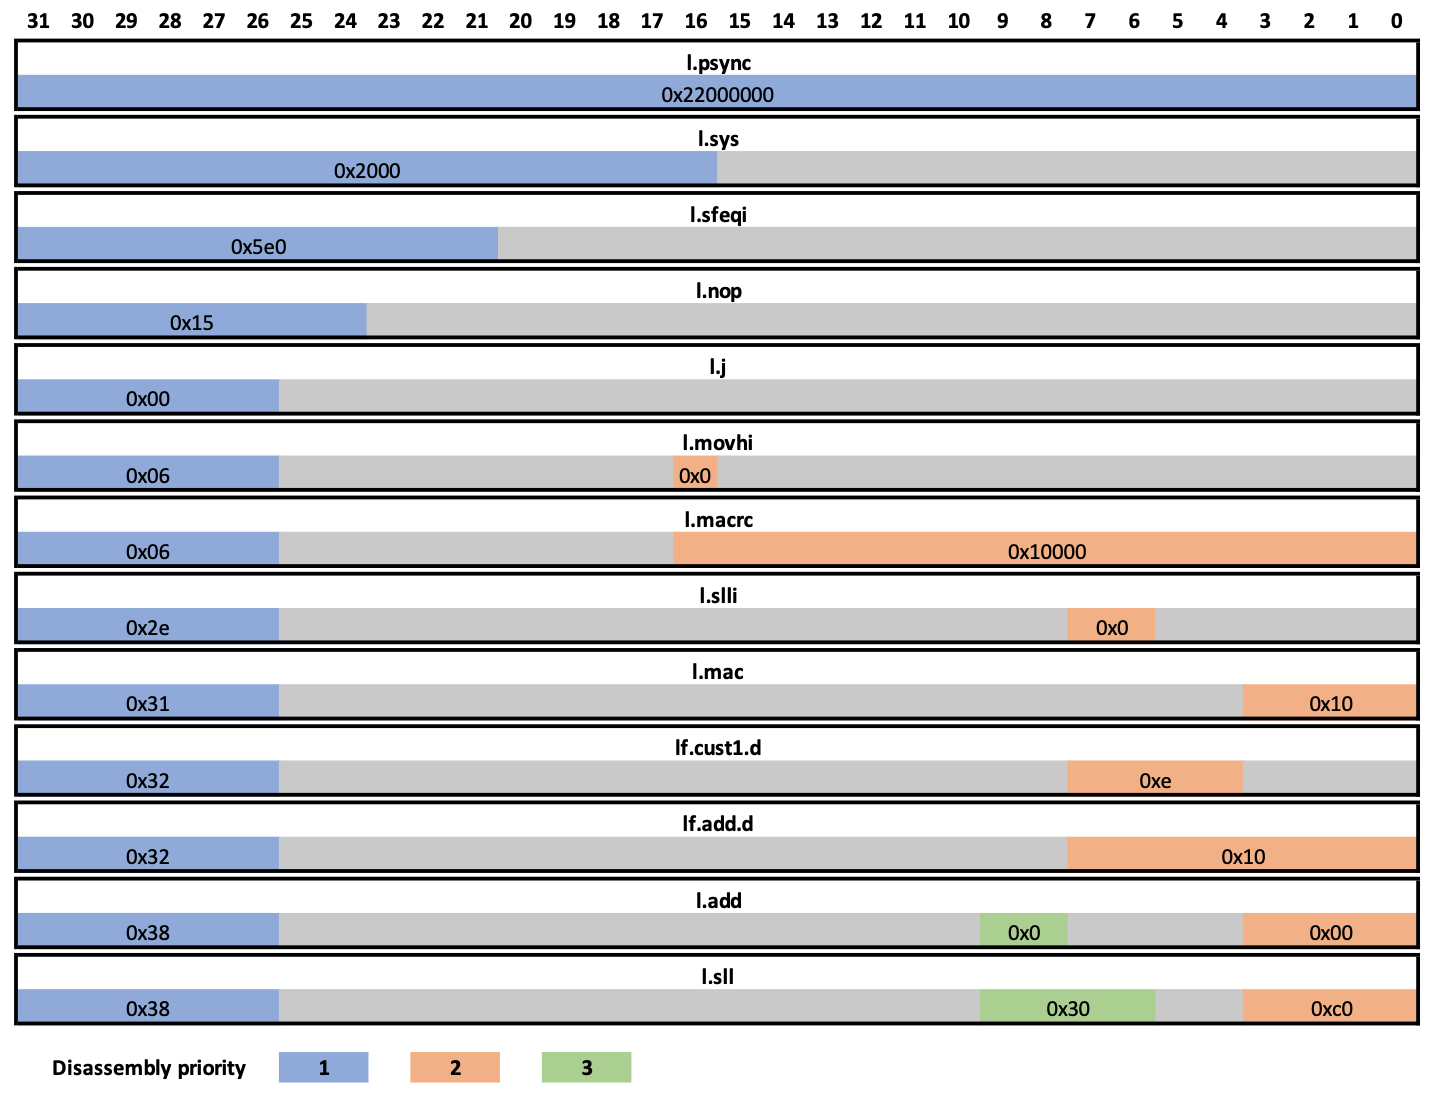
\includegraphics[width=\columnwidth]{diagrams/InstructionGroups}}
\caption{Skupiny inštrukcií podľa pozície operačného kódu}
\label{fig}
\end{figure}

\section{ELF súbory}

\section{Návrh implementácie}

\subsection{Algoritmus}

\subsection{Štruktúra aplikácie}

\begin{figure}[H]
\centerline{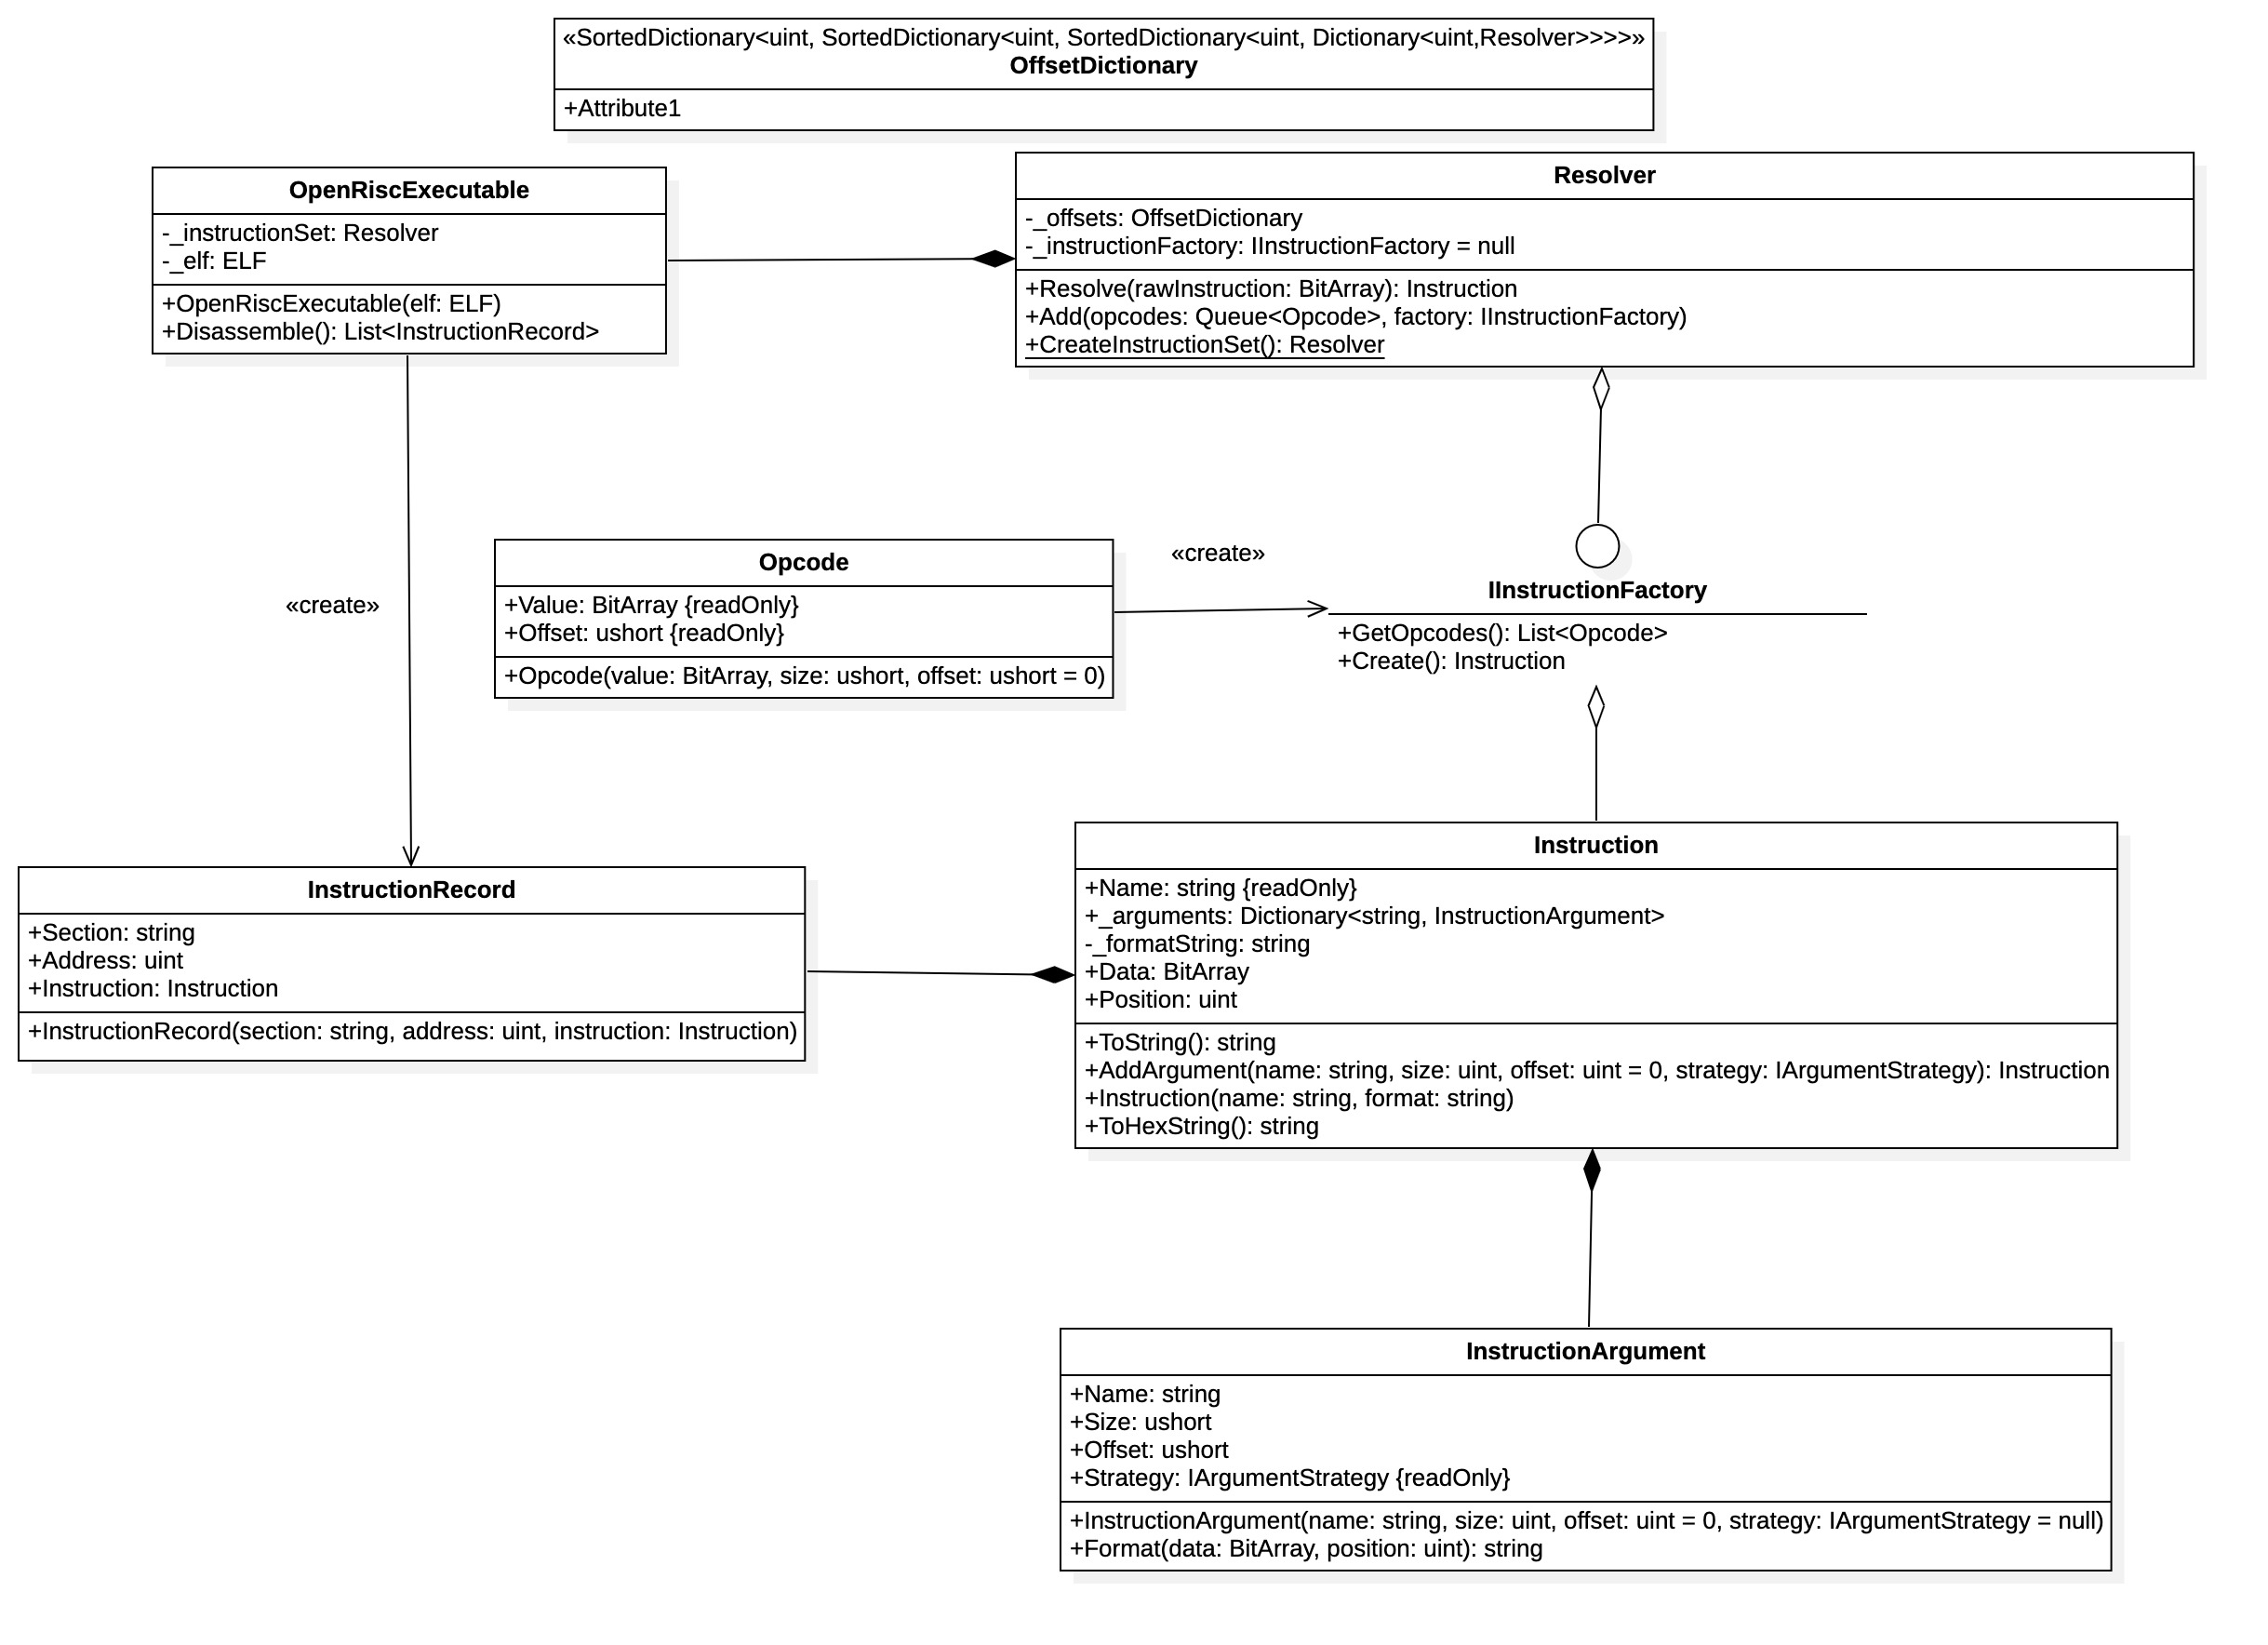
\includegraphics[width=\columnwidth]{diagrams/ClassDiagram}}
\caption{Example of a figure caption.}
\label{fig}
\end{figure}

\section{Zhodnotenie}

\bibliographystyle{IEEEtran}

\bibliography{my_bibs}

\end{document}